\section{Segmentation}
\subsection{Présentation de la méthode}
Tout d'abord, il nous a fallu considérer les images initialement fournies. Les images fournies sont des cartes de profondeur en niveaux de gris. Ces images se trouvaient être au format YML, représentées sous forme matricielle par des nombres flottants. N'ayant trouvé de méthode OpenCV permettant le chargement de ces fichiers, et afin de faciliter le travail sur ces images, nous avons choisi de convertir les fichiers .YML originaux en fichier .BMP. Pour ce faire, nous avons développé une fonction permettant de charger les fichiers originaux, puis d'effectuer une conversion sur les données contenues afin de les rentre compatible avec leur utilisation dans le cadre d'une image. Ainsi, nous avons tenté plusieurs conversions différentes afin de transformer les nombres flottants originaux pour obtenir des valeurs comprises entre 0 et 255. 

Nous avons tout d'abord tenté une interpolation linéaire des valeurs originales. La formule de conversion était alors :

\[
255 \times \frac{val - min}{max - min}
\]

avec $va$l le nombre flottant original, $min$ la valeur minimale du fichier YML, $max$ la valeur maximale du fichier YML.

\begin{figure}[htb!]
\centerline{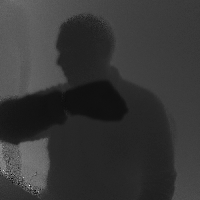
\includegraphics{interpLineaire.png}}
\caption{Résultat de l'interpolation linéaire des valeurs flottantes de l'image source.}
\label{fig:interpLineaire}
\end{figure}

Considérant ce résultat peu satisfaisant (\autoref{fig:interpLineaire}), nous avons tenté une seconde interpolation, basée non plus sur le minimum et maximum, mais sur la moyenne des valeurs du fichier YML original. Ainsi, la formule devint :

\[
255\times\frac{val}{moy}
\]

\begin{figure}[htb!]
\centerline{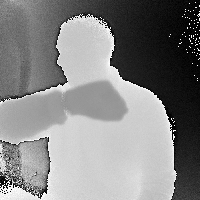
\includegraphics{interpMoyenne.png}}
\caption{Résultat de l'interpolation basée sur la moyenne des valeurs.}
\label{fig:interpMoyenne}
\end{figure}

A nouveau peu satisfait du résultat (\autoref{fig:interpMoyenne}), nous avons tenté une troisième formule, avec un résultat élevé au carré afin de privilégier les zones foncées dont la main fait partie, au détriment des zones claires peu intéressantes dans notre cas (\autoref{fig:interpQuadratique}). La conversion s'effectuait alors par :

\[
(val \times 16)^2
\]

\begin{figure}[htb!]
\centerline{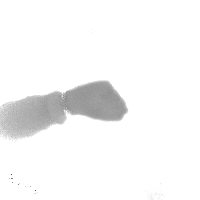
\includegraphics{interpQuadratique.png}}
\caption{Résultat de la conversion quadratique.}
\label{fig:interpQuadratique}
\end{figure}

La première étape de travail consiste à traiter les images initiales afin d’en extraire la zone d’intérêt à savoir ici la main. Travaillant sur des images de profondeur à une seule composante, la segmentation ne représente pas ici une étape compliquée du processus de traitement de l’image, mais ne peut non plus se borner à un simple seuillage binaire. En effet, dans la mesure où la main n’est pas toujours idéalement positionnée, mais sa distance à la caméra variant d’une image à l’autre, il est nécessaire de seuiller automatiquement l’image. En ce sens et après plusieurs tests et quelques recherches, il s’est avéré que l’algorithme de Fisher répondait très bien à la problématique posée.

	Etant disponible et efficace dans la librairie Pandore, nous avons entrepris d’utiliser cette dernière, ou tout du moins l’opérateur Fisher afin de ne pas redévelopper un algorithme implémenté de manière optimale. L’opérateur permet entre autre d’effectuer un multi-seuillage sur l’image et de répartir ses pixels selon les seuils déterminés.

\begin{figure}[htb!]
\centerline{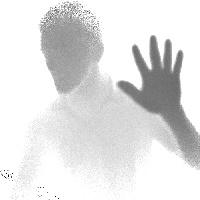
\includegraphics[scale=0.6]{fisherIn.jpg}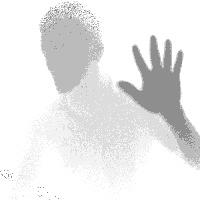
\includegraphics[scale=0.6]{fisherOut.jpg}}
\caption{Image source et seuillée avec Fisher.}
\end{figure}

Comme on peut le constater, l’algorithme distribue les pixels selon n classes distinctes, n étant un paramètre de l’algorithme. Ce dernier a été fixé à 5 pour apporter des résultats optimaux sur le plus grand nombre d’images.

	Une fois le multi-seuillage réalisé, nous bénéficions d’une image sur laquelle les pixels occupent n des 256 niveaux de gris. Partant du postulat que dans la plupart des cas présentés, l’élément à extraire se trouve en avant-plan de l’image de profondeur, cela signifie que la classe de pixels représentant cet élément est la plus sombre. Bien sûr, cela n’est pas une généralité et cela se vérifie uniquement lorsque la main est bien l’élément le plus sombre de l’image de profondeur, mais nous souhaitions tout d’abord avoir une bonne segmentation, efficace dans la majorité des cas présentés. 

La seconde partie de la segmentation consiste à égaliser l’histogramme. De la sorte, la première classe de pixels prend la valeur 0 et tous les pixels de la main deviennent donc noirs. On peut alors effectuer une seuillage binaire sur la valeur 0 pour ne garder que la main (\autoref{fig:resultatSeuillage}).

\begin{figure}[htb!]
\centerline{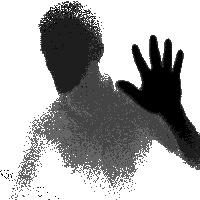
\includegraphics[scale=0.6]{thresholdIn.jpg} 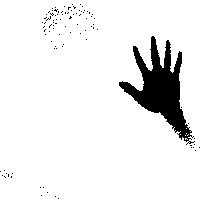
\includegraphics[scale=0.6]{thresholdOut.jpg}}
\caption{Entrée et sortie du seuillage binaire après égalisation de l'histogramme.}
\label{fig:resultatSeuillage}
\end{figure}

Comme on peut le constater sur les images ci-dessus, cette méthode n’est pas parfaite. Même si elle apporte des résultats confortables sur la plupart des images, elle rend en sortie une image sur laquelle on peut observer une quantité non négligeable de pixels résiduels. Nous avons donc développé une fonction de traitement permettant de « nettoyer » l’image et de supprimer l’ensemble de ces pixels épars qui ne font pas partie d’une composante connexe. Le principe est simple : Nous étudions la connexité de chaque pixel, afin de déterminer s’il appartient à un regroupement de pixels et donc s’il doit être supprimé.

Considérant $d_{inf}(P,Q)$, la distance de l’échiquier entre les points $P$ et $Q$, on appelle voisinage d’ordre $k$ du pixel $P$, l’ensemble des pixels $Q$ définit par : 

\[
V_k(P) = Q \text{tels que $0 < d_{inf}(P,Q) < k$}
\]

Considérant l’ordre de connexité $8$, $V_1$ représente donc l’ensemble des $8$ voisins directs, soit le plus petit voisinage non vide d’un pixel. L’opérateur de traitement consiste à supprimer un pixel $P$ lorsque le nombre de pixels de la même couleur que $P$ dans $V_1$, est inférieur à une certaine limite notée $\alpha$.  C'est-à-dire que pour le pixel considéré, il faut au moins $\alpha$ pixels noirs dans la zone colorée en vert dans l’image ci-dessous (\autoref{fig:pixelConnexite8}).

\begin{figure}[htb!]
\centerline{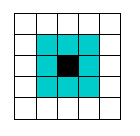
\includegraphics{connexite8.png}}
\caption{Pixel connexité 8.}
\label{fig:pixelConnexite8}
\end{figure}

Après une batterie de tests, cette limite a été fixée à $5$. En dessous, la main peut être entièrement supprimée après application du traitement, tandis qu’au dessus, certains pixels gênants pour la reconnaissance peuvent être laissés sur l’image. L’opérateur est appliqué plusieurs fois, ce qui permet d'opérer une érosion du poignet, gênant pour la reconnaissance. L’histogramme de l’image est inversé avant application de l’opérateur. Voici ci-dessous, le résultat de la segmentation sur la première image du groupe $1$ (\autoref{fig:segmentationGrp1}).

\begin{figure}
\centerline{
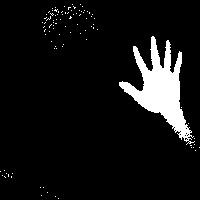
\includegraphics[scale=0.6]{segIn.jpg}

\includegraphics[scale=0.6]{segOut.jpg}
}
\caption{Résultat de la segmentation pour la première image du groupe $1$, avant et après filtrage.}
\label{fig:segmentationGrp1}
\end{figure}

\subsection{Analyse des résultats}
Cette méthode de segmentation se trouve être efficace sur la majorité des images fournies dans la base. Voici un panel de test réalisé sur l’ensemble des images du groupe $1$ :

\foreach \n in {2,3,5,6}{
\centerline{
\includegraphics[scale=0.6]{segIn\n.png}
\includegraphics[scale=0.6]{segOut\n.jpg}
}
}

Le taux de réussite s’avère très correct puisque 13 images sur 16 sont traitées correctement. On observe des erreurs dans deux cas : 
\begin{itemize}
\item Lorsqu’il n’y a pas de main ($2^{eme}$ image)
\item Lorsque la main n’est pas en avant-plan (images 1 et 4).
\end{itemize}

Dans les deux cas, l’algorithme doit être en mesure de détecter que l’étape de segmentation n’a pas été optimale, dans la mesure où la reconnaissance ne renverra pas de résultat. L’algorithme de segmentation ne peut cependant pas être corrigé simplement pour palier les problèmes et lorsqu’une main est effectivement présente dans l’image, il n’est actuellement pas en mesure de se focaliser sur cette dernière pour l’extraire. Une telle solution n’a pas été implémentée par manque de temps et également cela demeure un cas très particulier. En effet dans une application de suivi de la main et de reconnaissance de geste, il est évident que l’homme qui effectue les gestes va instinctivement placer les mains devant son corps et non l’inverse.

Sur une autre base d’images qu’est le groupe 3, certaines images posent problème lorsque le bras est placé perpendiculairement à l’axe de vision de la caméra, autrement dit lorsque le bras et la main sont à égale distance de la caméra (images de 13 à 18 dans le groupe). Le contraste de l’image s’avère alors très peu élevé et des pixels résiduels noirs, bien plus foncés que le membre à reconnaître faussent alors l’étape de segmentation.

Dans le tableau ci-dessous, on observe un test sur 3 images. Comme on peut l’observer, la segmentation sur les deux premières est loin de fournir un résultat satisfait exploitable par la reconnaissance, tandis que la dernière est segmentée « parfaitement » sans correction nécessaire. Une solution a consisté à nettoyer l’image en prétraitement, afin de supprimer les pixels résiduels sombres, faussant la segmentation sur 5 des 18 images du groupe 3. Seulement, comme on peut le constater, cette correction s’avère être néfaste sur des images sur laquelle la segmentation était initialement réussie. Nous n’avons à l’heure actuelle pas exploré de piste nous permettant de traiter idéalement et automatiquement toutes les images.

\begin{figure}
\begin{tabular}{|c|c|c|}
\hline
Image source & Image non corrigée avant segmentation & Image corrigée avant segmentation\\
\hline
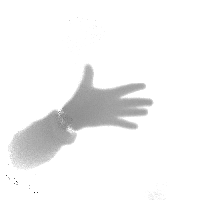
\includegraphics[scale=0.4]{correcSrc1.png} & 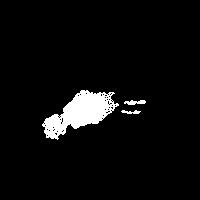
\includegraphics[scale=0.4]{correcOut1-1.jpg} & 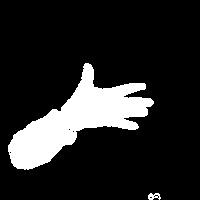
\includegraphics[scale=0.4]{correcOut2-1.jpg} \\
\hline
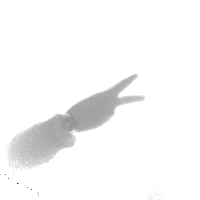
\includegraphics[scale=0.4]{correcSrc2.png} & 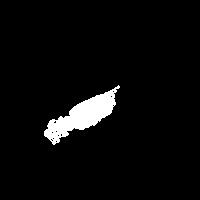
\includegraphics[scale=0.4]{correcOut1-2.jpg} & 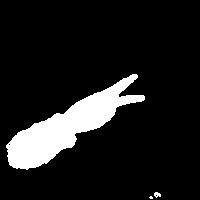
\includegraphics[scale=0.4]{correcOut2-2.jpg} \\
\hline
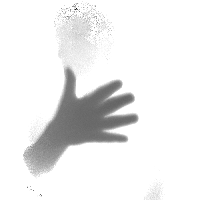
\includegraphics[scale=0.4]{correcSrc3.png} & 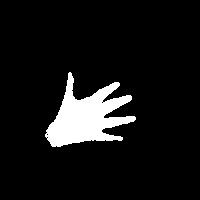
\includegraphics[scale=0.4]{correcOut1-3.jpg} & 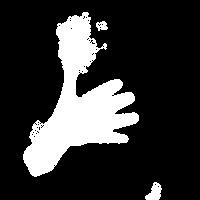
\includegraphics[scale=0.4]{correcOut2-3.jpg} \\
\hline
\end{tabular}
\caption{Résultats de la correction.}
\end{figure}

